\section{Experimentos e Resultados}

Nesta seção são apresentados os experimentos realizados para comparar as abordagens de controle de estilo por engenharia de \textit{prompts} e por \textit{fine-tuning} com LoRA. São descritas as configurações utilizadas, os critérios de avaliação e os resultados obtidos com base em métricas objetivas e análise qualitativa.

\subsection{Configuração Experimental}

Foram utilizados os \textit{prompts} com leves diferenças para os dois modelos, levando em conta que o modelo para engenharia de \textit{prompts} é generalista, ele precisa de entradas detalhadas e específicas para gerar as imagens de forma esperada, por exemplo ``\textit{A field of blooming wildflowers under a cloudy sky, painted in the impressionist style of Monet}'', enquanto, por outro lado, o ajuste com LoRA do outro modelo foi feito com o propósito de o modelo não precisar de especificações sobre o estilo, mas sim gerar sempre nesse estilo, com a entrada equivalente sendo ``\textit{A field of blooming wildflowers under a cloudy sky}'', omitindo detalhes sobre o estilo. A Tabela \ref{tab:prompts} mostra cada um dos \textit{prompts} utilizados.

\begin{table}[htb]
\caption{\textit{Prompts} para compara\c{c}\~ao entre os modelos com e sem \textit{fine-tuning}}
\centering
\begin{tabular}{p{0.47\textwidth} p{0.47\textwidth}}
\toprule
\textbf{\textit{Prompt} (modelo com LoRA)} & \textbf{\textit{Prompt} (modelo base com engenharia)} \\
\midrule
\textit{A calm lake at sunset} &
\textit{A calm lake at sunset, in the style of Claude Monet, with soft brushstrokes and warm impressionist tones} \\
\textit{A field of blooming wildflowers under a cloudy sky} &
\textit{A field of blooming wildflowers under a cloudy sky, painted in the impressionist style of Monet} \\
\textit{A small wooden bridge over a quiet river} &
\textit{A small wooden bridge over a quiet river, Claude Monet style, with light reflections and vibrant pastels }\\
\textit{A seaside village with boats on the shore }&
\textit{A seaside village with boats on the shore, impressionist painting, in Claude Monet's style }\\
\textit{A rainy street in a 19th-century European town} &
\textit{A rainy 19th-century European street, painted with dabs of color and soft outlines, in Claude Monet’s style} \\
\textit{A lush garden with rose arches and green hedges} &
\textit{A lush garden with rose arches and green hedges, in the style of Claude Monet, impressionist garden scene} \\
\textit{Snow-covered trees on a hill in winter }&
\textit{Snow-covered hill with trees, impressionist painting, soft brushwork, Claude Monet winter style} \\
\textit{A steam train passing through a countryside station} &
\textit{A steam train in a countryside station, impressionist style, inspired by Monet }\\
\textit{Sunset over calm ocean waves with orange glow }&
\textit{Sunset over ocean, impressionist style with glowing pastels, Claude Monet inspired }\\
\textit{A forest path in early autumn} &
\textit{A forest path in early autumn, impressionist colors and diffuse lighting, Monet style} \\
\bottomrule
\end{tabular}
\label{tab:prompts}
\fonte{Autoria pr\'opria}
\end{table}

Os \textit{prompts} foram utilizados para gerar 10 imagens distintas em cada modelo, com 20 imagens geradas no total, variando a semente aleatória para promover diversidade. As imagens geradas foram então avaliadas segundo critérios de fidelidade ao estilo impressionista e consistência visual.

\subsection{Métricas de Avaliação}

A avaliação objetiva foi conduzida por meio das seguintes métricas:

\begin{itemize}
    \item \textbf{CLIPScore}~\cite{clipscore}: mede a compatibilidade semântica entre o prompt textual e a imagem gerada, baseado nas embeddings do modelo CLIP.
    \item \textbf{FID (\textit{Fréchet Inception Distance})}~\cite{fid}: avalia a distância entre as distribuições de características extraídas das imagens geradas e reais, usando o Inception v3. Quanto menor o valor, maior a similaridade.
\end{itemize}

Além disso, foi realizada uma análise qualitativa visual das imagens, observando aspectos como pinceladas, uso de cor e composição, características típicas do estilo de Claude Monet.

\subsection{Resultados Quantitativos}

A Tabela~\ref{tab:clipscore_duplo} apresenta os valores de CLIPScore para os dois modelos (base e \textit{fine-tuned} com LoRA), considerando dois cenários de avaliação: com o \textit{prompt} original utilizado na geração da imagem e com um \textit{prompt} padronizado contendo descrições estilísticas associadas a Claude Monet. A média de CLIPScore usando os \textit{prompts} originais foi de 30.04 para o modelo base e 32.95 para o modelo LoRA, indicando que o \textit{fine-tuning} contribuiu para uma maior fidelidade semântica às descrições fornecidas, mesmo sem menções explícitas ao estilo impressionista durante a geração. Encontra-se uma visualização gráfica desses dados na Figura \ref{fig:clipscore}

Ao se utilizar o prompt estilizado com termos como ``\textit{impressionist style}'' e ``\textit{in the style of Claude Monet}'', os resultados se invertem: o modelo base obteve uma média superior (34.81) em relação ao modelo LoRA (31.23). Esse resultado indica que o modelo base responde melhor quando há instruções textuais explícitas sobre o estilo de Monet, enquanto o modelo LoRA foi treinado para expressar o estilo aprendendo diretamente das imagens, sem depender de instruções textuais. Ou seja, o modelo LoRA gera imagens mais coerentes com \textit{prompts} neutros, mas não necessariamente se alinha melhor com descrições textuais ricas em estilo, já que esse viés já está internalizado em sua representação visual.

Além disso, a métrica FID entre os dois conjuntos de imagens foi de 305.10, indicando uma grande diferença visual entre as imagens geradas pelos modelos. Este valor reforça que o \textit{fine-tuning} com LoRA resultou em imagens com características visuais significativamente distintas — e mais próximas ao estilo de Monet — em comparação ao modelo base. Em conjunto, os resultados apontam que o \textit{fine-tuning} com LoRA não apenas melhora a fidelidade semântica em \textit{prompts} genéricos, mas também altera substancialmente o espaço visual do modelo para capturar o estilo-alvo, mesmo sem instruções explícitas.

\begin{table}[htb]
\caption{CLIPScore com prompt original e com estilo Monet para os dois modelos}
\centering
\begin{tabular}{p{4.5cm}cccc}
\toprule
\textbf{Prompt} & \textbf{Base (orig)} & \textbf{LoRA (orig)} & \textbf{Base (Monet)} & \textbf{LoRA (Monet)} \\
\midrule
A calm lake at sunset & 24.34 & 30.81 & 31.62 & 32.02 \\
A field of blooming wildflowers under a cloudy sky & 30.17 & 32.85 & 31.83 & 31.71 \\
A small wooden bridge over a quiet river & 28.18 & 33.59 & 35.01 & 34.28 \\
A seaside village with boats on the shore & 29.71 & 31.79 & 32.60 & 31.17 \\
A rainy street in a 19th-century European town & 35.91 & 38.15 & 37.27 & 34.21 \\
A lush garden with rose arches and green hedges & 30.02 & 36.83 & 36.74 & 33.52 \\
Snow-covered trees on a hill in winter & 29.80 & 30.17 & 36.67 & 25.61 \\
A steam train passing through a countryside station & 30.84 & 30.78 & 35.69 & 24.84 \\
Sunset over calm ocean waves with orange glow & 30.54 & 31.35 & 35.46 & 34.02 \\
A forest path in early autumn & 30.87 & 33.22 & 35.19 & 30.92 \\
\midrule
\textbf{Média} & 30.04 & 32.95 & 34.81 & 31.23 \\
\bottomrule
\end{tabular}
\label{tab:clipscore_duplo}
\fonte{Autoria própria}
\end{table}

\begin{figure}
    \centering
    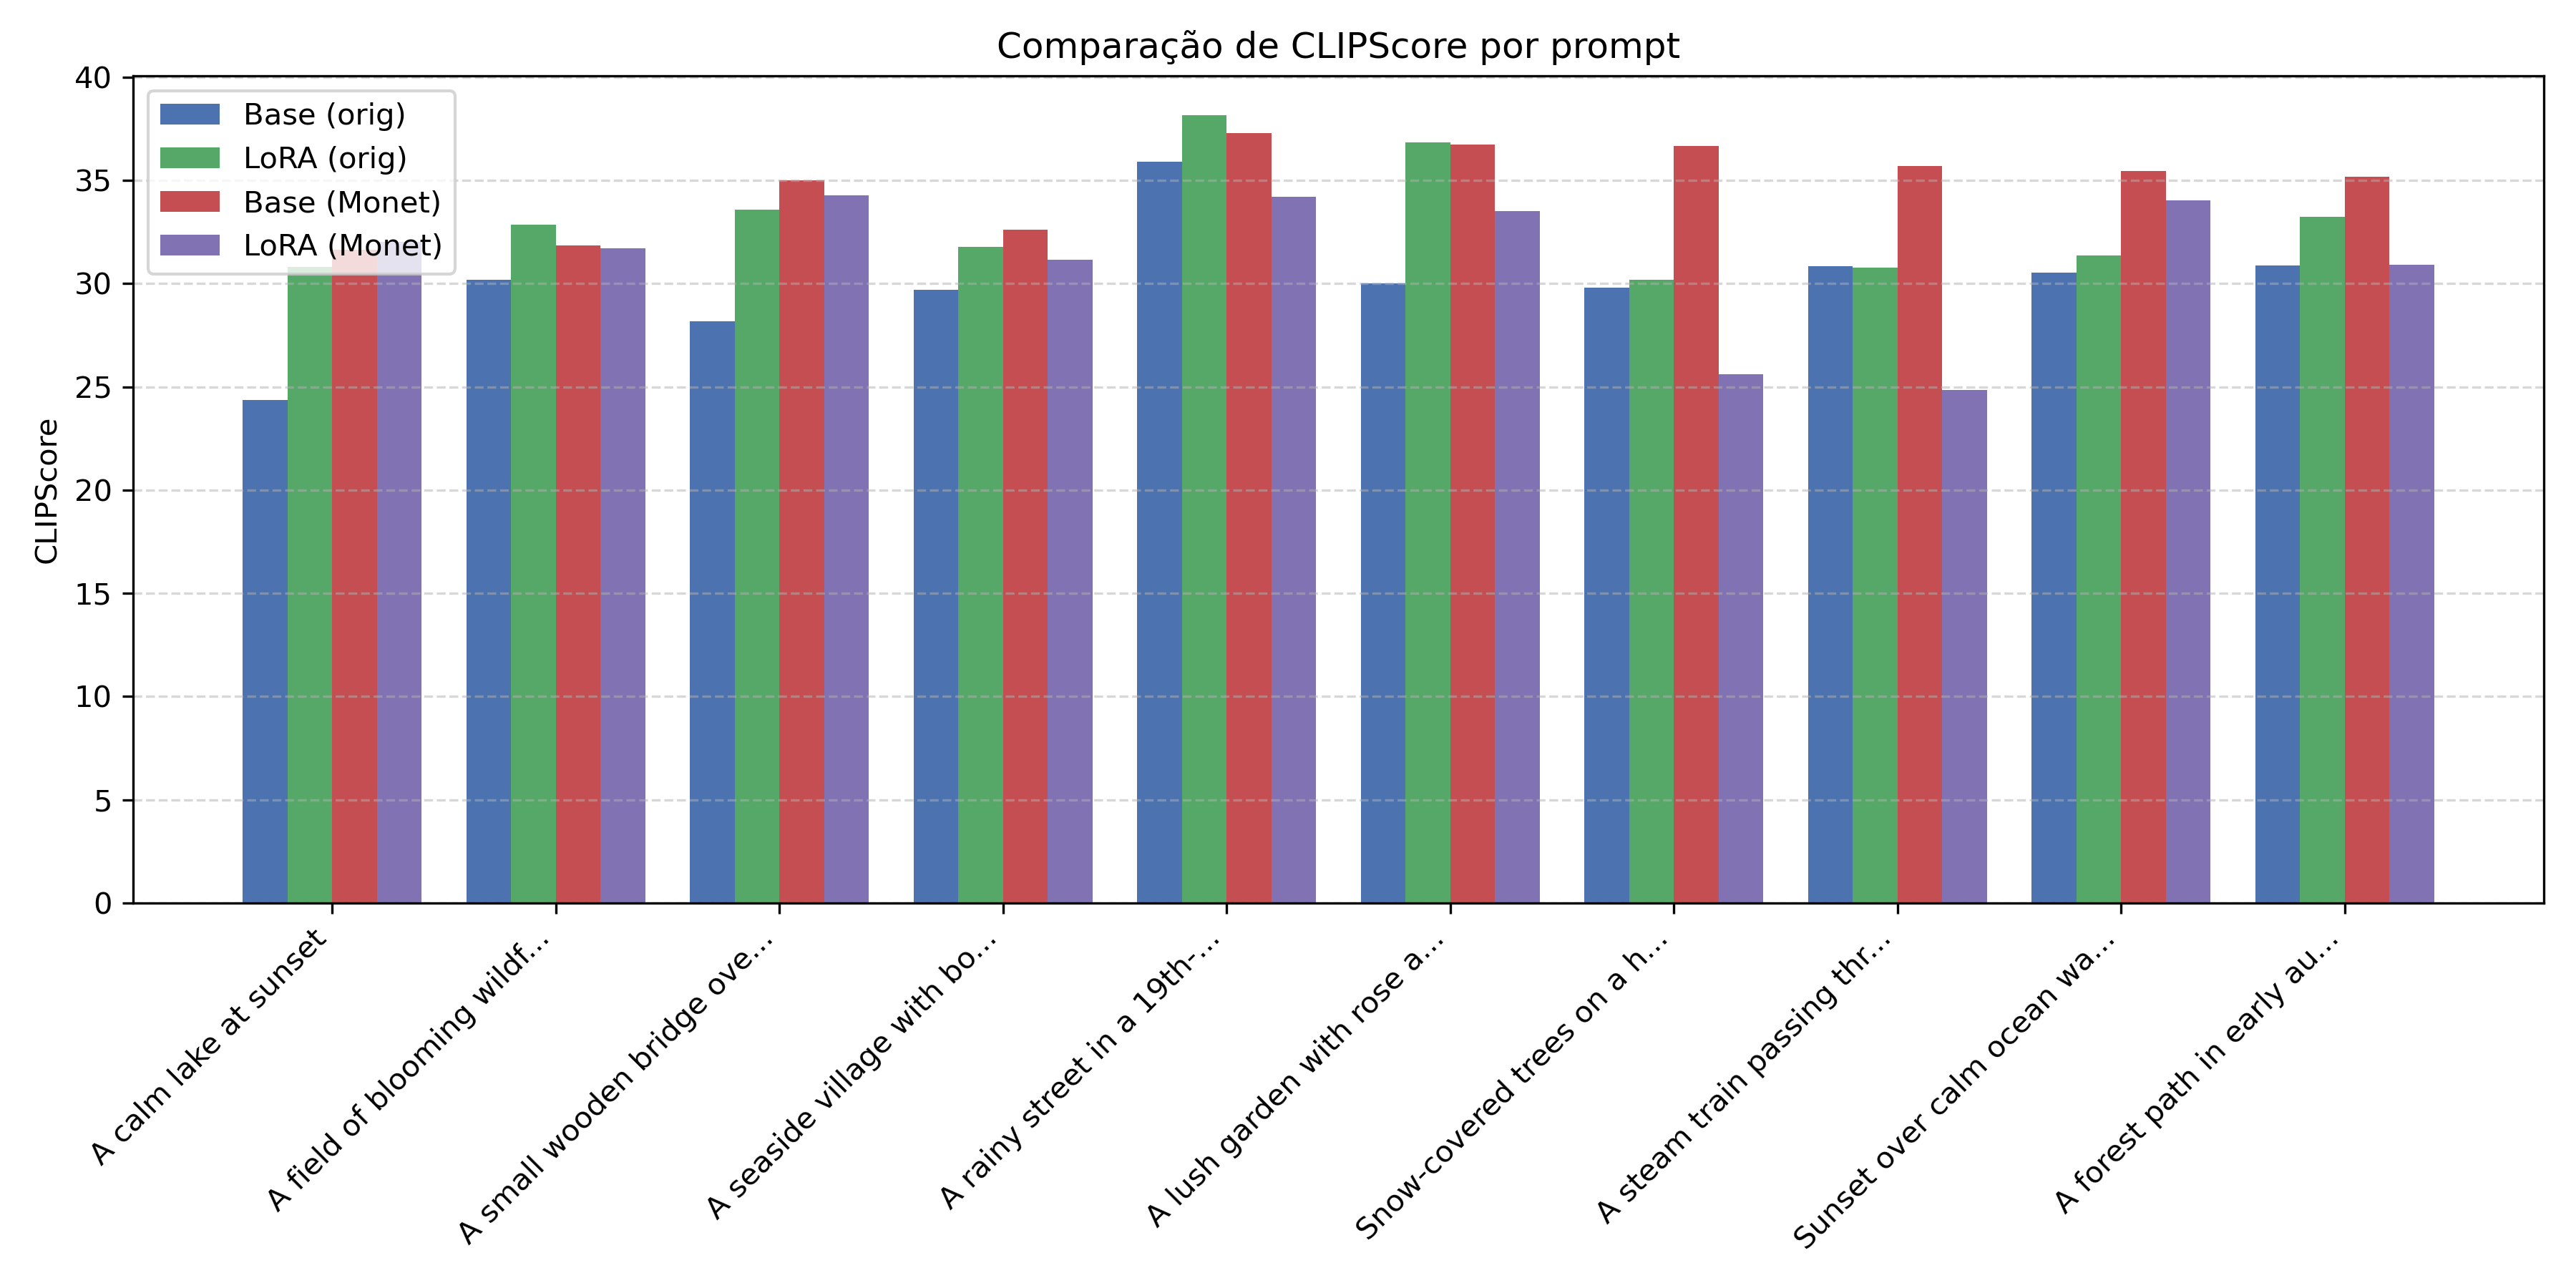
\includegraphics[width=1\linewidth]{clipscore_comparacao.png}
    \caption{Representação gráfica dos CLIPScores}
    \label{fig:clipscore}
    \fonte{Autoria própria}
\end{figure}

\subsection{Análise Qualitativa}

As Figuras~\ref{fig:analise_qualitativa_part1} e \ref{fig:analise_qualitativa_part2} apresentam uma comparação visual entre amostras geradas pelas duas abordagens. Observa-se que o modelo \textit{fine-tuned} com LoRA demonstra dificuldade em manter o estilo de Monet em alguns exemplos, como o do \textit{prompt} ``\textit{A steam train passing through a countryside station}'', onde ele adota um estilo mais próximo do realismo. Isso reflete a ausência de trens no \textit{dataset} de pinturas de Monet, resultando na falta de representação de objetos do tipo, fazendo com que o modelo opte pela representação já aprendida em sua versão base.

As imagens geradas pelo modelo base, por outro lado, representam uma visão uniformizada do estilo impressionista de Monet, podendo ser explicado pelo fato de hoje o autor ser um grande representante do movimento impressionista, quando na verdade as pinturas do autor incluíam outros estilos variados não necessariamente impressionistas, melhor representados na coluna das imagens geradas com o modelo ajustado com LoRA

As imagens geradas pela abordagem de engenharia de \textit{prompts} demonstram maior capacidade de generalização do estilo, refletindo a flexibilidade da técnica, embora limitada pela falta de especialização do modelo. A abordagem com LoRA, por outro lado, denota maior fidelidade ao estilo do autor, porém com uma notável dificuldade em generalizar o seu estilo para aplicações novas.

\begin{figure}[htb]
\centering
\caption{Análise qualitativa (Parte 1): imagens geradas por ambos os modelos para cada \textit{prompt}}
\label{fig:analise_qualitativa_part1}

\begin{tabular}{p{4.5cm}c@{\hskip 0.5cm}c}
\toprule
\textbf{\textit{Prompt}} & \textbf{Base} & \textbf{LoRA} \\
\midrule

A calm lake at sunset &
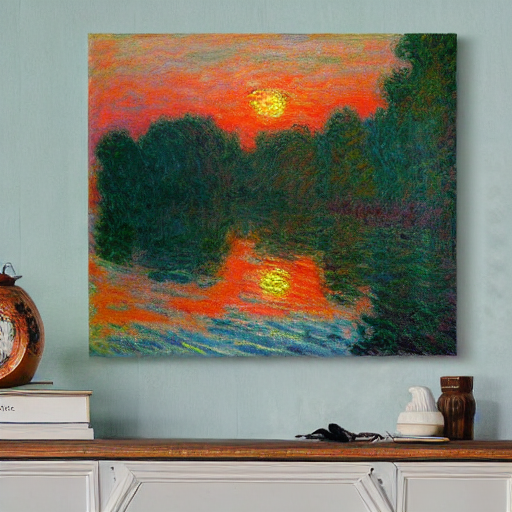
\includegraphics[width=0.25\linewidth]{modelo_base/01_a_calm_lake_at_sunset.png} &
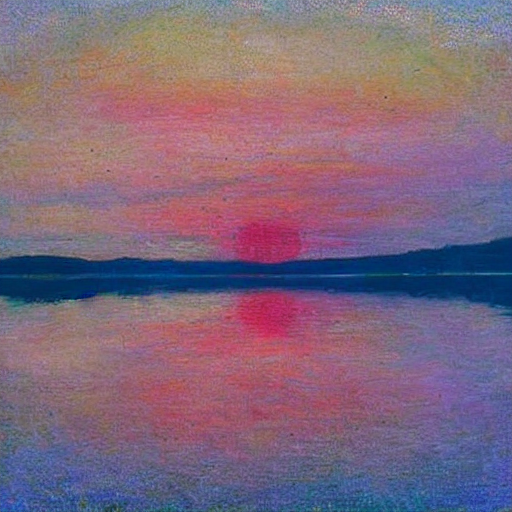
\includegraphics[width=0.25\linewidth]{modelo_lora/01_a_calm_lake_at_sunset.png} \\

A field of blooming wildflowers under a cloudy sky &
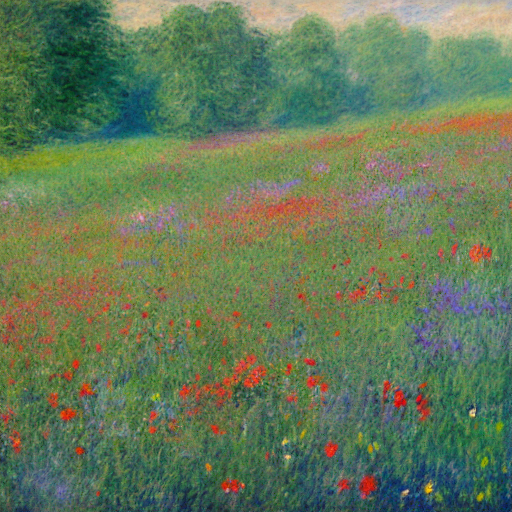
\includegraphics[width=0.25\linewidth]{modelo_base/02_a_field_of_blooming_wildflower.png} &
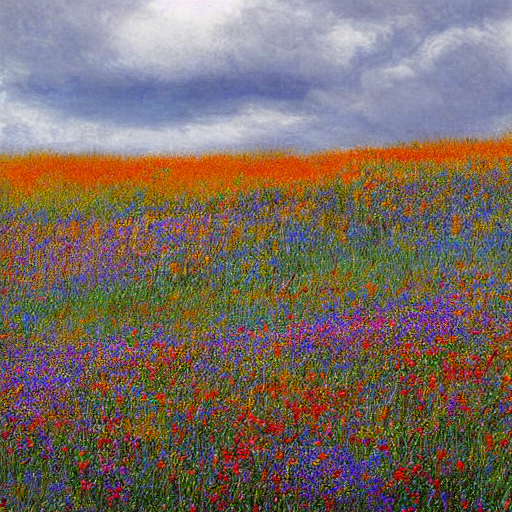
\includegraphics[width=0.25\linewidth]{modelo_lora/02_a_field_of_blooming_wildflower.png} \\

A small wooden bridge over a quiet river &
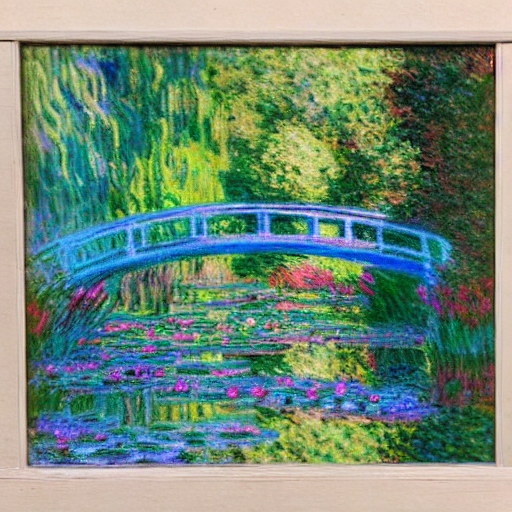
\includegraphics[width=0.25\linewidth]{modelo_base/03_a_small_wooden_bridge_over_a_q.png} &
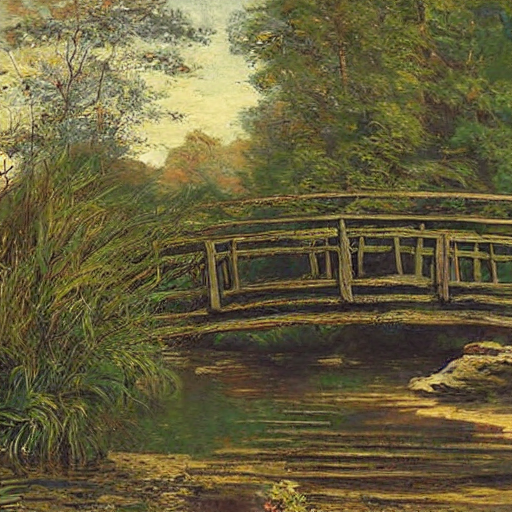
\includegraphics[width=0.25\linewidth]{modelo_lora/03_a_small_wooden_bridge_over_a_q.png} \\

A seaside village with boats on the shore &
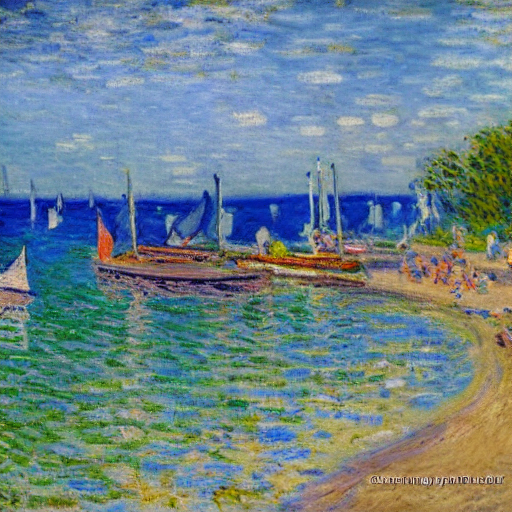
\includegraphics[width=0.25\linewidth]{modelo_base/04_a_seaside_village_with_boats_o.png} &
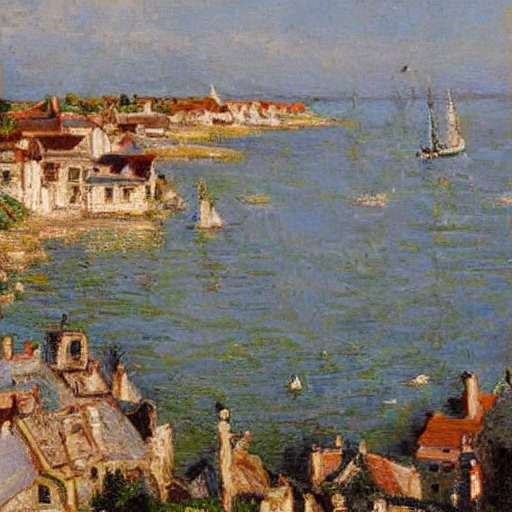
\includegraphics[width=0.25\linewidth]{modelo_lora/04_a_seaside_village_with_boats_o.png} \\

A rainy street in a 19th-century European town &
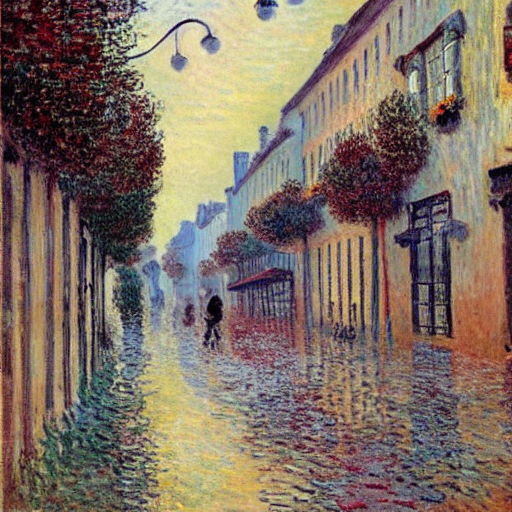
\includegraphics[width=0.25\linewidth]{modelo_base/05_a_rainy_street_in_a_19th-centu.png} &
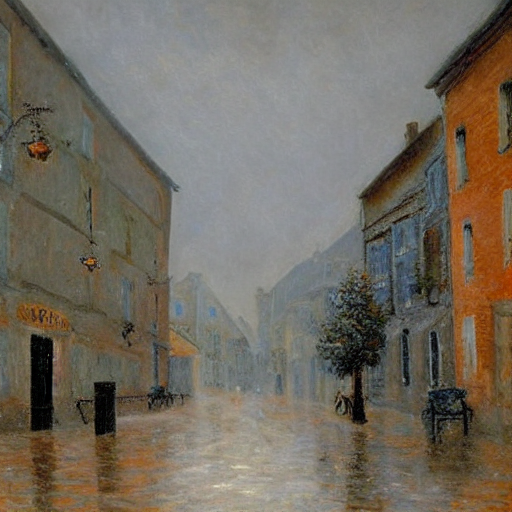
\includegraphics[width=0.25\linewidth]{modelo_lora/05_a_rainy_street_in_a_19th-centu.png} \\

\bottomrule
\end{tabular}
\fonte{Autoria própria}
\end{figure}


\begin{figure}[htb]
\centering
\caption{Análise qualitativa (Parte 2): imagens geradas por ambos os modelos para cada \textit{prompt}}
\label{fig:analise_qualitativa_part2}

\begin{tabular}{p{4.5cm}c@{\hskip 0.5cm}c}
\toprule
\textbf{\textit{Prompt}} & \textbf{Base} & \textbf{LoRA} \\
\midrule

A lush garden with rose arches and green hedges &
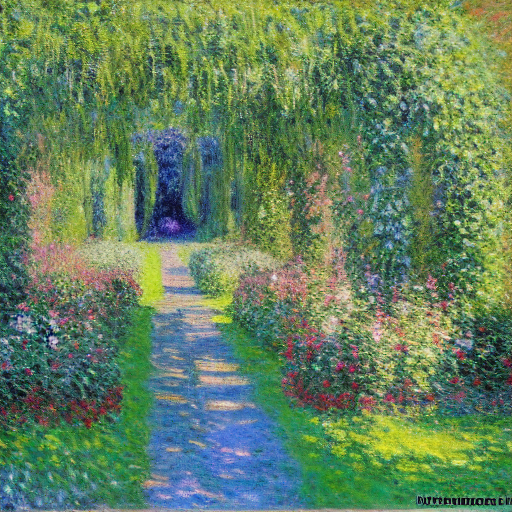
\includegraphics[width=0.25\linewidth]{modelo_base/06_a_lush_garden_with_rose_arches.png} &
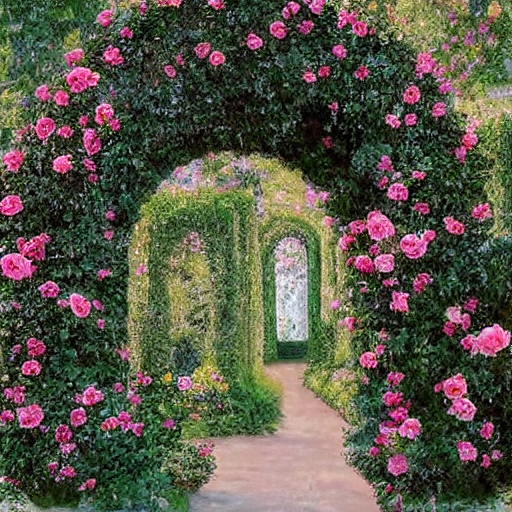
\includegraphics[width=0.25\linewidth]{modelo_lora/06_a_lush_garden_with_rose_arches.png} \\

Snow-covered trees on a hill in winter &
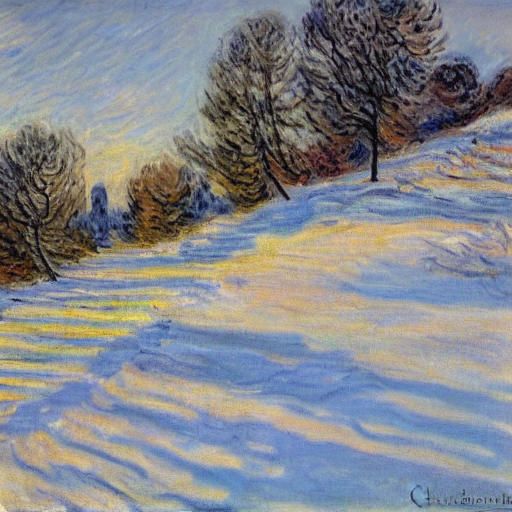
\includegraphics[width=0.25\linewidth]{modelo_base/07_snow-covered_trees_on_a_hill_i.png} &
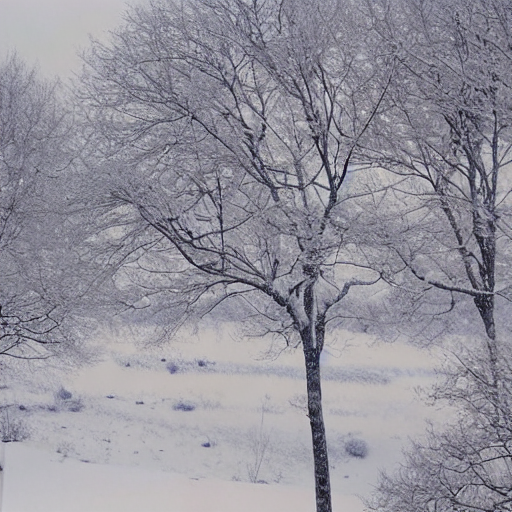
\includegraphics[width=0.25\linewidth]{modelo_lora/07_snow-covered_trees_on_a_hill_i.png} \\

A steam train passing through a countryside station &
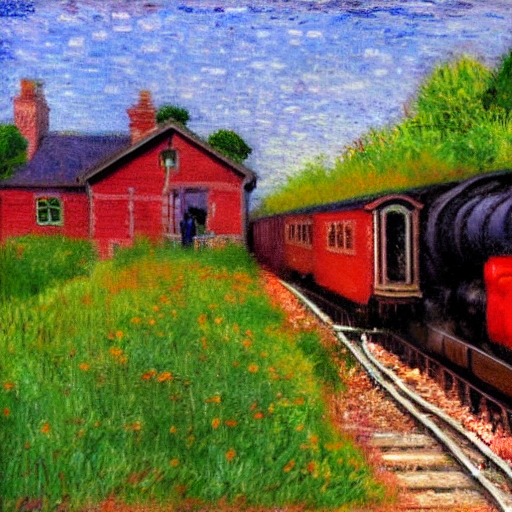
\includegraphics[width=0.25\linewidth]{modelo_base/08_a_steam_train_passing_through_.png} &
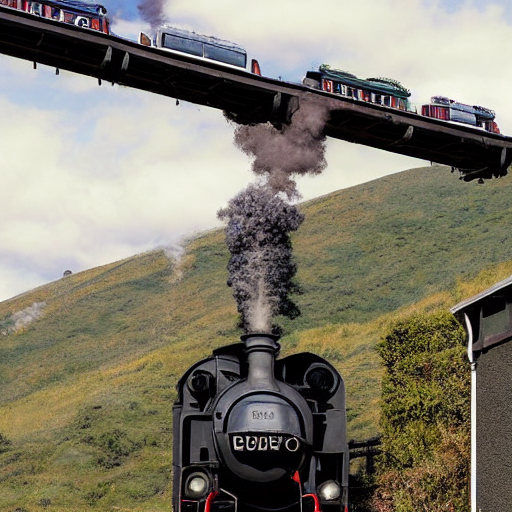
\includegraphics[width=0.25\linewidth]{modelo_lora/08_a_steam_train_passing_through_.png} \\

Sunset over calm ocean waves with orange glow &
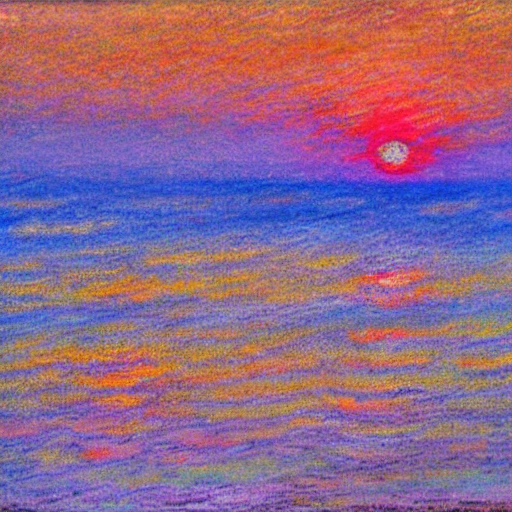
\includegraphics[width=0.25\linewidth]{modelo_base/09_sunset_over_calm_ocean_waves_w.png} &
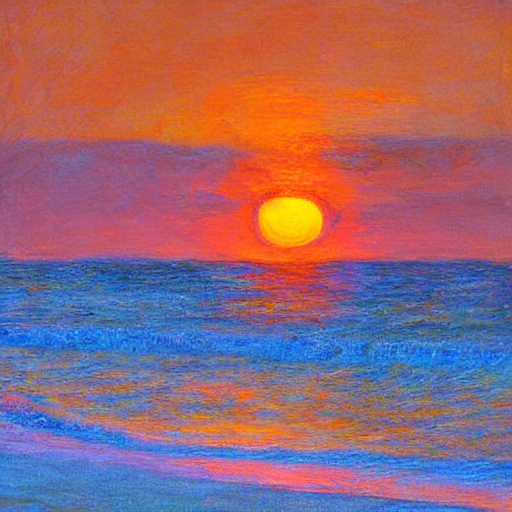
\includegraphics[width=0.25\linewidth]{modelo_lora/09_sunset_over_calm_ocean_waves_w.png} \\

A forest path in early autumn &
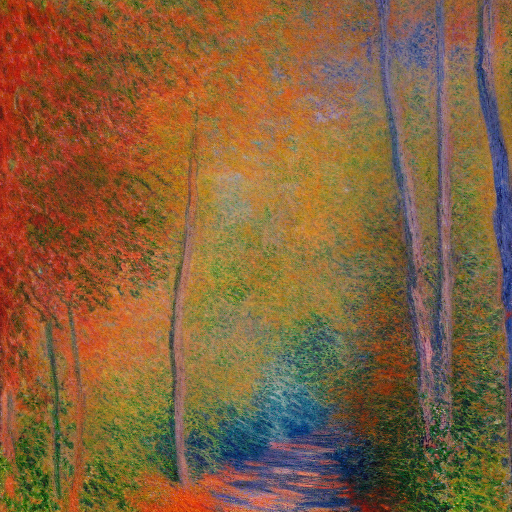
\includegraphics[width=0.25\linewidth]{modelo_base/10_a_forest_path_in_early_autumn.png} &
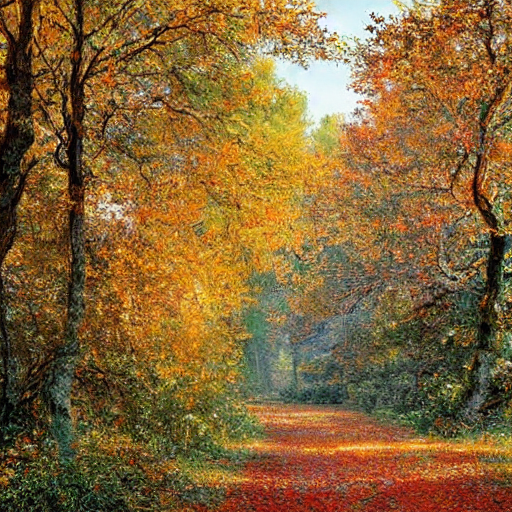
\includegraphics[width=0.25\linewidth]{modelo_lora/10_a_forest_path_in_early_autumn.png} \\

\bottomrule
\end{tabular}
\fonte{Autoria própria}
\end{figure}